\subsection{Gameplay Elements}

In this section we will see in more detail all the aspect that make this video games unique in its genre. The game is a 2D single player third person game, the player will play with the character of Minerva, both in her human form and in "cat" form. The combat is turn-based and the formulation of the player's stats are based on the D\&D rules.

%TODO
\paragraph{Exploration Mode}

The player is free to move around  the map in both human form that cat form. If Delphini is also in the player's party, she will follow the player in his every move, but if he is in cat form and enters a place not accessible to humans, Delphini will remain waiting for him When the player is faced with a obstacle, mysterious object or secret passage, he can: 

\begin{itemize}
    \item Use the spells that he has learning to solve the puzzle.
    \item Has the possibility of being able to use the transfiguration to transform small objects into somethings that is needed at the moment.
    \item Transform into cat form and reach places inaccessible to human.
\end{itemize}

The player can interact with NPCs:

\begin{itemize}
    \item In human form he can talk to them, they can make funny story or riddles.
    \item In cat form he can be stroked.
\end{itemize}

\fullwidthgraphicscaption{../Pictures/Gameplay/Dialogue_picture.jpg}{Game: Doom\&Destiny}

\pagebreak 

\paragraph{Combat System}
The combat is turn based. It mostly follows D\&D rules, only exception being that space and movement don't play any role: the combat happens like an old school sideview turn-based rpg. All the D\&D rules that involve moving around don't play any role. Area spells and skills will hit multiple enemies without checking an on-map position. Finally maximum range values for ranged spells and attacks will not play any role.

The main reason is increasing the pace of the fight, since a more complex system which involves movement, getting closer to the turn-based strategy games paradigm, would be too slow paced and complex for the ideal target audience.

\fullwidthgraphicscaption{../Pictures/Gameplay/Combat_picture.png}{Game: Octopath traveler}
\pagebreak

\paragraph{Player rewards}

The player's reward are obtainable in every fight. In the specific combat with Cerberus the player can get: 60 Galleon, 80 Sickle and 100 Knut

\centeredgraphicssize{../Pictures/Gameplay/Rewards_picture.jpg}{5cm}

\paragraph{Experience Points and Friendship Points}

Characters gain Experience Points by completing challenges, missions and minigames (lessons). When Experience Points reach a certain treshold, the Character's level rises. 
Each level grants all the spells of that level which have already been seen during a lesson.

Delphini has an stat in Frienship Points. These increase and decrease depending on the player's choices and successes in missions involving Delphini.

When Delphini is in the party and the friendship level is low, Delphini has access to more aggressive spells, up to Forbidden Curses. 
In contrast, if the friendship level is high, when Minerva attacks Delphini will use a reaction action to perform an attack toghether with Minerva.


\paragraph{Gryffindor Points}

When the player completes a task really well (perfect score in minigames, extremely good timing in timed tasks etcc) or when he fails terribly, some points are added to or removed from the player's House Points. Sometimes player choices can affect the points of other houses as well.
Grants an achievement on the chosen game platform if Gryffindor has the highest points by the end of the game.

\pagebreak 

\paragraph{Checkpoints}

Checkpoints are save points where the player can go back after a defeat. They appear as a Niffler statue which activates when the player makes an offer with a special coine called "Niffler Galleon".
\centeredgraphicssize{../Pictures/Gameplay/Statue_niffler_picture.jpg}{5cm}

\paragraph{Saving}

Checkpoints also save the game. The player can still save at anytime through the main menu. During battles saving is disabled.
\pagebreak

\subsubsection{Items}

\paragraph{Key Items}

\textbf{Key Items}\\

\begin{itemize}
    \item \textbf {Cauldron} 
A tool required in order to prepare potions. A portable version costs 25 galleons, which allows the player to brew potions anywhere. It's magically enchanted to shrink itself so to be easily carried around.
\centeredgraphicssize{../Pictures/Gameplay/Items/Cauldron_picture.png}{5cm}
 
   \item \textbf{Book of Spells }   
A book worth 2 galleons, is used to keep track of the learnt spells.
\centeredgraphicssize{../Pictures/Gameplay/Items/Book_spells_picture.png}{5cm}
   
 \item \textbf{Book of Potions}
 A book worth 2 galleons, is used to keep track of the learnt potion.
\centeredgraphicssize{../Pictures/Gameplay/Items/Book_potions_picture.png}{5cm}
\end{itemize}
\pagebreak



\pagebreak
\paragraph{Consumables}
For consumables we intend all the items that can be used directly or through a crafting process: inside of this category we can find currency, ingredients and craftables. \\
\subparagraph{Currency}

\begin{tabular}{m{3cm}m{3cm}m{6cm} } \hline
	
\includegraphics[width=3cm]{../Pictures/Gameplay/Items/Consumables/Currency/Knut_coin_picture.png} & \textbf{Knut} & A Knut, made out of bronze, is the least valued coin in British wizarding currency. There are 29 Knuts in one silver Sickle, and there are 493 Knuts in one golden Galleon. \\ \hline
	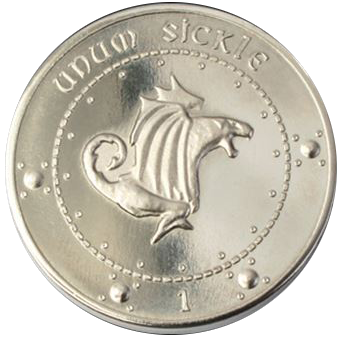
\includegraphics[width=3cm]{../Pictures/Gameplay/Items/Consumables/Currency/Sickle_coin_picture.png} & \textbf{Sickle} & A Sickle, made out of silver, is equal to 29 Knuts, and 17 Sickles make up a Galleon. \\ \hline
	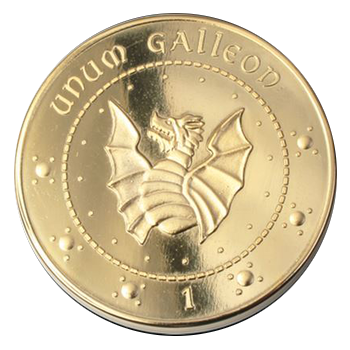
\includegraphics[width=3cm]{../Pictures/Gameplay/Items/Consumables/Currency/Galleon_coin_picture.png} & \textbf{Galleon} & A Galleon, made out of gold, is the most valued coin of the wizarding currency used in Britain. One Galleon is equal to 17 Sickles or 493 Knuts.  \\ \hline
	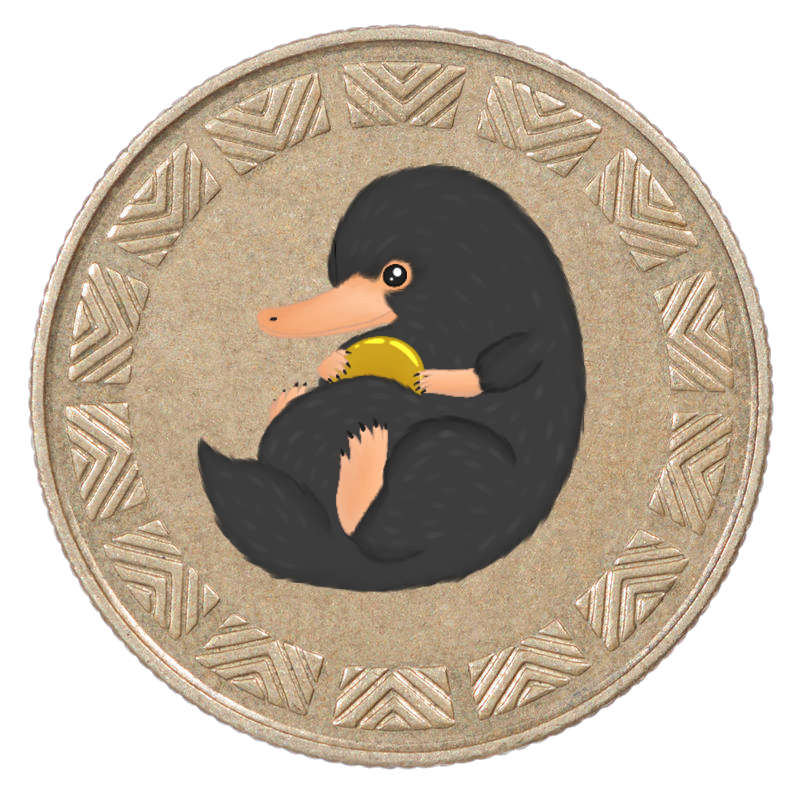
\includegraphics[width=3cm]{../Pictures/Gameplay/Items/Consumables/Currency/Niffler_coin_front_picture.png} & \textbf{Niffler Galleon} & Special currency, grants the blessing of the Niffler when used at their statues, acting as an effective checkpoint for the player. \\ \hline
\end{tabular}

\clearpage


\subparagraph{Ingredients}
Ingredients are plants or other elements useful for potion-making.

\begin{tabular}{m{2cm}m{3cm}m{10cm} } 
	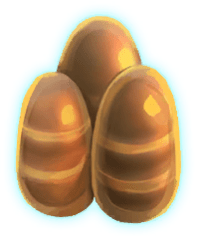
\includegraphics[width=2cm]{../Pictures/Gameplay/Items/Consumables/Ingredients/Ashwinder_eggs_picture.png} & \textbf{Ashwinder Egg} & Ashwinder eggs are the eggs of the Ashwinder , a magical serpent  which is born from the embers of an unattended magical fire. \\ 
	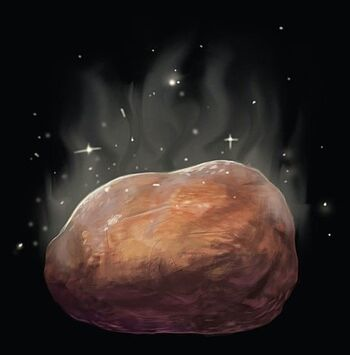
\includegraphics[width=2cm]{../Pictures/Gameplay/Items/Consumables/Ingredients/Bezoar_picture.png} & \textbf{Bezoar} & A bezoar is a stone-like mass taken from the stomach of a goat, that acts as an antitode to most potions \\ 
	
\includegraphics[width=2cm]{../Pictures/Gameplay/Items/Consumables/Ingredients/Bitter_root_picture.png} & \textbf{Bitter Root} & Bitter root (alternatively spelled bitterroot) is a plant that can be used as a potion ingredient. \\ 
	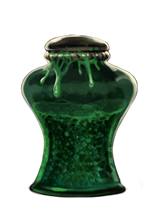
\includegraphics[width=2cm]{../Pictures/Gameplay/Items/Consumables/Ingredients/Flobberworm_mucus_picture.png} & \textbf{Flobberworm Mucus} & Flobberworm mucus, alternatively spelled Flobberworm mucous or Flobber Mucus for short, is the slimy green mucus exuded from the Flobberoworm, often used to thicken potions. \\ 
	
\includegraphics[width=2cm]{../Pictures/Gameplay/Items/Consumables/Ingredients/Granian_hair_picture.png} & \textbf{Granian Hair} & Granian hair is hair taken from a Granian Winged horse, which can be used as a potion ingredient. \\ 
	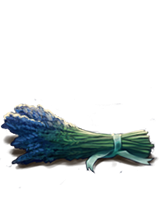
\includegraphics[width=2cm]{../Pictures/Gameplay/Items/Consumables/Ingredients/Lavender_picture.png} & \textbf{Lavender} & Lavender is a flower noted for its "beautiful colour" and "calming fragrance. It can be used as an ingredient in a variety of potions. \\ 
	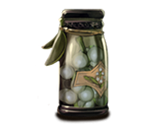
\includegraphics[width=2cm]{../Pictures/Gameplay/Items/Consumables/Ingredients/Mistletoe_berries_picture.png} & \textbf{Mistletoe Berries} & The berry of the mistletoe is small, white, and waxy. It is used as an ingredient in potion. \\ 
	
\includegraphics[width=2cm]{../Pictures/Gameplay/Items/Consumables/Ingredients/Murtlap_tentacle_picture.png} & \textbf{Murtlap Tentacle} & A Murtlap tentacle is a rare potion ingredient that can be obtained from the growth on the back of a Murtlap. \\ 
	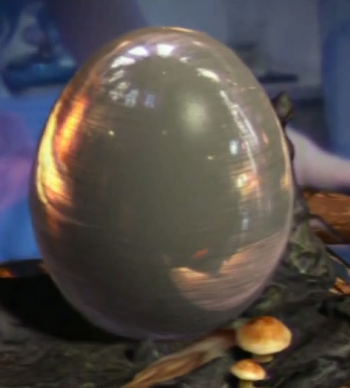
\includegraphics[width=2cm]{../Pictures/Gameplay/Items/Consumables/Ingredients/Occamy_egg_picture.png} & \textbf{Occamy Eggshell} & The egg of the Occamy has a shell made of pure silver, which accounts for why it is so much sought after. \\ 
	
\includegraphics[width=2cm]{../Pictures/Gameplay/Items/Consumables/Ingredients/Reem_blood_picture.png} & \textbf{Re'em Blood} & Re'em blood gives the drinker immense strength for a short time. This in turn makes Re'em blood a highly desired substance, and a useful potion ingredient. \\ 
	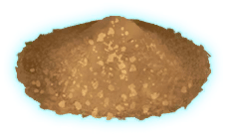
\includegraphics[width=2cm]{../Pictures/Gameplay/Items/Consumables/Ingredients/Rue_picture.png} & \textbf{Rue} & Rue, also known as common rue, is a kind of evergreen shrubs with a distinctive bitter taste. \\ 
	
\includegraphics[width=2cm]{../Pictures/Gameplay/Items/Consumables/Ingredients/Snowdrop_picture.png} & \textbf{Snowdrop} & This plant is very well known for its stimulant properties. \\ 
\end{tabular}

\clearpage

\begin{tabular}{m{2cm}m{3cm}m{10cm} } 
	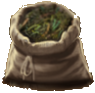
\includegraphics[width=2cm]{../Pictures/Gameplay/Items/Consumables/Ingredients/Standard_ingredient_picture.png} & \textbf{Standard Ingredient} & The Standard Ingredient is a herb, or mixture of dried herbs, with many magical applications and properties that is used as an ingredient in potion-making.  \\ 
	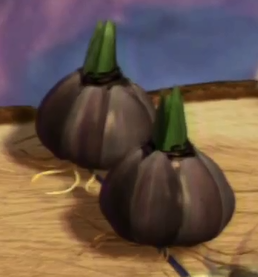
\includegraphics[width=2cm]{../Pictures/Gameplay/Items/Consumables/Ingredients/Squill_bulbs_picture.png} & \textbf{Squill Bulbs} & The bulb of the squill is a structure that functions as an organ for food storage while the plant is dormant. Squill bulbs have potion-making properties and are best harvested just after the plants blossoms. \\ 
	
\includegraphics[width=2cm]{../Pictures/Gameplay/Items/Consumables/Ingredients/Tincture_of_thyme_picture.png} & \textbf{Tincture of Thyme} & Thyme is a common herb with culinary and medicinal uses, making it a good candidate for potion-making. \\ 
	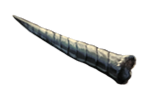
\includegraphics[width=2cm]{../Pictures/Gameplay/Items/Consumables/Ingredients/Unicorn_horn_picture.png} & \textbf{Unicorn Horn} & The horn of a unicorn had magical properties that made it a useful ingredient in potions. \\ 
	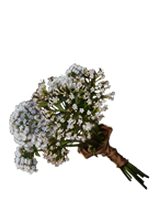
\includegraphics[width=2cm]{../Pictures/Gameplay/Items/Consumables/Ingredients/Valerian_picture.png} & \textbf{Valerian Sprigs} & Valerian is a plant with magical and calming properties. \\ 
\end{tabular}

\clearpage

\subparagraph{Craftables}
Objects made with ingredients\\

\begin{itemize}
    \item \textbf{Antidote common poisons}
 Neutralizes poisonous effects from magical creatures. Can be used both in battle and outside.
 Ingredients: Bezoar, Standard Ingredient, Unicorn Horn, Mistletoe Berries.
\centeredgraphicssize{../Pictures/Gameplay/Items/Consumables/Potions/Antidote_potion_picture.png}{5cm}
    
    \item \textbf{Exstimulo Potion}
Increases the power of spells casted in the next 4 turns.
Ingredients: Re'em blood, Granian hair, Snowdrop and Bitter root
\centeredgraphicssize{../Pictures/Gameplay/Items/Consumables/Potions/Exstimulo_potion_picture.png}{5cm}

    \item \textbf{Felix Felicis}
Makes who drinks it extremely lucky. Combat rewards are increased, healing potions effect is increased, and all rolls are rolled with advantage.
Ingredients: Ashwinder egg, Squill builb, Murtlap tentacle, Tincture of thyme, Occamy eggshell, Powdered common rue.
\centeredgraphicssize{../Pictures/Gameplay/Items/Consumables/Potions/Felix_felicis_potion_picture.png}{5cm}
    
	\item \textbf{Healing Potion}
 Recovers health points. This potion's effect varies based on the amount of ingredients used to prepare it. %TODO: how many ingredients define normal/medium/superior?

\begin{tabular}{ |c|c|c } 
\hline
\textbf{Rarity} & \textbf{HP}  & \textbf{Ingredients Amount} \\
\hline
Normal  & 2d4  & 1  \\
\hline
Medium  & 4d4 & 3 \\
\hline
Superior  & 8d4 & 5 \\
\hline
\end{tabular}

\centeredgraphicssize{../Pictures/Gameplay/Items/Consumables/Potions/Healing_potion_picture.png}{5cm}

	 \item \textbf{Invisibility Potion}
Makes the user invisible. In battle the potion lasts 3 turns, out of battle it lasts one minute. The potion affects the user and everything he's carrying; it terminates when the user attacks, casts a spell, or shifts form.
Ingredients: Flobberworm Mucus, Lavender, Valerian Sprigs, Standard ingredient
\centeredgraphicssize{../Pictures/Gameplay/Items/Consumables/Potions/Invisibility_potion_picture.png}{5cm}
\end{itemize}
\pagebreak

\paragraph{Wands}
\textbf{Wands} In Hogwarts, everything is based on wizardry and spells: for this reason the wand, together with protective jewelry, will play an important role in combat, enhancing the magical capabilities of our characters in different ways.

The wand is the most important tool in a wizard's life: inner magical power is channeled through it and it can cast any kind of spell. Each wand is made of wood and contains an enchanted core, a special material usually coming from magical creatures.
\centeredgraphicssize{../Pictures/Gameplay/Items/Wand_picture.jpg}{5cm}
There are several types of wand wood and cores, which will alter and enhance the capabilities of the wielder.

\paragraph{Wood} The wood will grant a bonus to its particular category of spells: \\

\begin{tabular}{ m{4cm}m{3cm}m{6cm} } \hline
	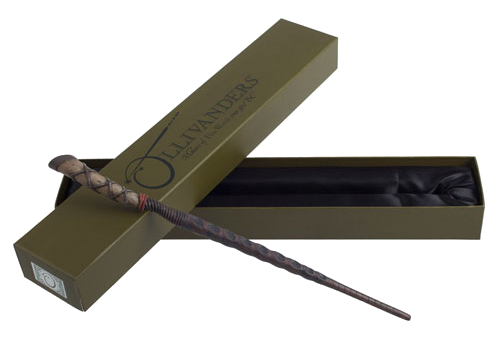
\includegraphics[width=4cm]{../Pictures/Gameplay/Items/Wearables/Wand/Wood/Holly_wood_picture.png} & \textbf{Holly} & Holly will boost defensive spells, naturally meant for casters who think that a good defense is the best offense. \\ \hline
	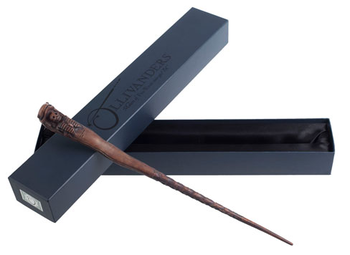
\includegraphics[width=4cm]{../Pictures/Gameplay/Items/Wearables/Wand/Wood/Alder_wood_picture.png} & \textbf{Alder} & Alder will boost buff spells, aiding mages who seek to help and empower others. \\ \hline
	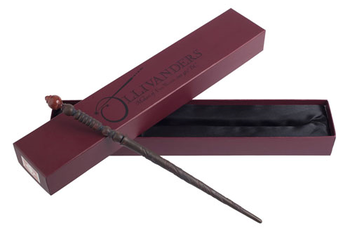
\includegraphics[width=4cm]{../Pictures/Gameplay/Items/Wearables/Wand/Wood/Cedar_wood_picture.png} & \textbf{Cedar} & Cedar will boost debuff spells, perfect for wizards who prefer to weaken their enemies before striking.  \\ \hline
	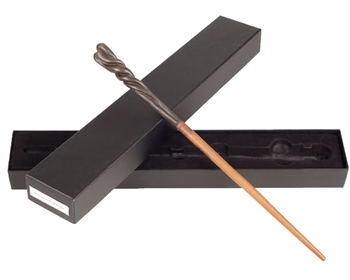
\includegraphics[width=4cm]{../Pictures/Gameplay/Items/Wearables/Wand/Wood/Cherry_wood_picture.png} & \textbf{Cherry} & Cherry will boost attack spells, favored by sorcerers who follow the rule "strike first, strike hard". \\ \hline
	
\includegraphics[width=4cm]{../Pictures/Gameplay/Items/Wearables/Wand/Wood/Pine_wood_picture.png} & \textbf{Pine} & Pine will boost utility spells, preferred by creative enchanters and out-of-the-box thinkers. \\ \hline
\end{tabular}
\pagebreak 
\begin{itemize}
    \item The bonus for non-Utility category will make spells of that category cast as 1 level higher (if applicable).
    \item The bonus for Utility category will grant an extra spell slot reserved to Utility spells for each spell level the character has access to.
\end{itemize}

\clearpage


\paragraph{Cores}
Cores will grant an unique bonus feat \\

\begin{tabular}{ m{4cm}m{3cm}m{6cm} } \hline
	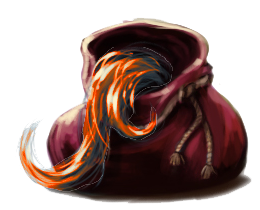
\includegraphics[width=4cm]{../Pictures/Gameplay/Items/Wearables/Wand/Cores/Dragon_heartstring_icon.png} & \textbf{Dragon Heartstring (Dual wielder)} & You can equip a second wand. You get the bonus from the wood of that wand, but not from its core. \\ \hline
	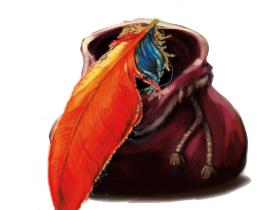
\includegraphics[width=4cm]{../Pictures/Gameplay/Items/Wearables/Wand/Cores/Phoenix_feather_icon.png} & \textbf{Phoenix Feather (Alert)} & Adds +5 to Initiative. \\ \hline
	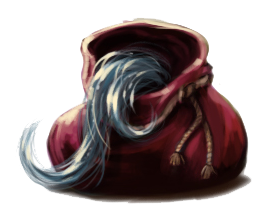
\includegraphics[width=4cm]{../Pictures/Gameplay/Items/Wearables/Wand/Cores/Unicorn_hair_icon.png} & \textbf{Unicorn Hair (Resilient)} & Adds +1 in one ability score and you gain proficiency in saving throws using that ability.  \\ \hline
	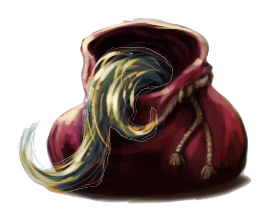
\includegraphics[width=4cm]{../Pictures/Gameplay/Items/Wearables/Wand/Cores/Veela_hair_icon.png} & \textbf{Veela Hair (Healer)} & You can stabilize a creature and restore it to 1 hp, or restore [1d6+4+its number of Hit Dice] hp to it; can't be used more than once per day on the same creature. \\ \hline
	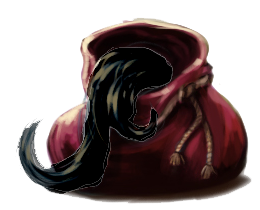
\includegraphics[width=4cm]{../Pictures/Gameplay/Items/Wearables/Wand/Cores/Thestral_tail_hair_icon.png} & \textbf{Thestral Tail Hair (Lucky)} & You can reroll a d20 or force to reroll an attack roll against you. Can be used up to 3 times per day. \\ \hline
\end{tabular}

\clearpage

\paragraph{Amulets}
Amulets will enhance ability scores \\

\begin{tabular}{m{2cm}m{3cm}m{4cm} } 
	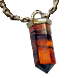
\includegraphics[width=2cm]{../Pictures/Gameplay/Items/Wearables/Amulets/Amber_amulet_icon.png} & \textbf{Amber} & adds +1 STR \\ 
	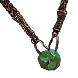
\includegraphics[width=2cm]{../Pictures/Gameplay/Items/Wearables/Amulets/Jade_amulet_icon.png} & \textbf{Jade} & adds +1 DEX \\ 
	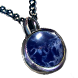
\includegraphics[width=2cm]{../Pictures/Gameplay/Items/Wearables/Amulets/Lapis_amulet_icon.png} & \textbf{Lapis} & adds +1 INT \\ 
	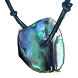
\includegraphics[width=2cm]{../Pictures/Gameplay/Items/Wearables/Amulets/Paua_amulet_icon.png} & \textbf{Paua} & adds +1 WIS \\ 
	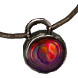
\includegraphics[width=2cm]{../Pictures/Gameplay/Items/Wearables/Amulets/Coral_amulet_icon.png} & \textbf{Coral} & adds +1 CON \\ 
	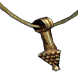
\includegraphics[width=2cm]{../Pictures/Gameplay/Items/Wearables/Amulets/Gold_amulet_icon.png} & \textbf{Gold} & adds +1 CHA \\ 
	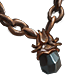
\includegraphics[width=2cm]{../Pictures/Gameplay/Items/Wearables/Amulets/Onyx_amulet_icon.png} & \textbf{Onyx} & (Rare), adds +1 to all ability scores 
\end{tabular}

\clearpage

\paragraph{Rings}

Rings will grant an unique bonus to the wearer. One can wear maximum two rings at once.
\begin{itemize}

    \item \textbf{Paua},  gives 1 additional spell slot, usable by any spell of any level
\centeredgraphicssize{../Pictures/Gameplay/Items/Wearables/Rings/Paua_ring_icon.png}{5cm}

  \item \textbf{Coral}, adds +8 HP
\centeredgraphicssize{../Pictures/Gameplay/Items/Wearables/Rings/Coral_ring_icon.png}{5cm}

  \item \textbf{Moonstone}, adds +2 on CA and +2 on Saving Throws when defending against spell attacks.
\centeredgraphicssize{../Pictures/Gameplay/Items/Wearables/Rings/Moonstone_ring_icon.png}{5cm}

  \item \textbf{Diamond} , adds +2 CA when defending against physical attacks.
\centeredgraphicssize{../Pictures/Gameplay/Items/Wearables/Rings/Diamond_ring_icon.png}{5cm}

\end{itemize}
\pagebreak

\subsubsection{Characters}

\fullwidthgraphics{../Pictures/Characters/Stat_sheets/Minerva_sheet.png}

\fullwidthgraphics{../Pictures/Characters/Stat_sheets/Delphini_sheet.png}

\fullwidthgraphics{../Pictures/Characters/Stat_sheets/Cerberus_sheet.png}
\pagebreak

\subsubsection{Enemies Chart}
\fullwidthgraphics{../Pictures/Story/Enemies_chart.jpg}